\documentclass[letterpaper,11pt]{article}
\usepackage{graphicx}
\usepackage{listings}
\usepackage[super]{nth}

\lstset{
	basicstyle=\footnotesize,
	breaklines=true,
}

\begin{document}

\begin{titlepage}

\begin{center}

\Huge{Assignment 2}

\Large{CS 595:  Introduction to Web Science}

\Large{Spring 2016}

\Large{Manoj Chandra Kompalli}

\Large Finished on February 11,2016

\end{center}

\end{titlepage}
\tableofcontents
\newpage




\section{Question 1}
\label{part1}
\begin{verbatim}
1.  Write a Python program that extracts 1000 unique links from
Twitter.  You might want to take a look at:

http://thomassileo.com/blog/2013/01/25/using-twitter-rest-api-v1-dot-1-with-python/

But there are many other similar resources available on the web.  Note
that only Twitter API 1.1 is currently available; version 1 code will
no longer work.

Also note that you need to verify that the final target URI (i.e., the
one that responds with a 200) is unique.  You could have many different
shortened URIs for www.cnn.com (t.co, bit.ly, goo.gl, etc.).

You might want to use the search feature to find URIs, or you can
pull them from the feed of someone famous (e.g., Tim O'Reilly).

Hold on to this collection -- we'll use it later throughout the semester.
\end{verbatim}
\newpage
\subsection{Answer}
I have started off by searching for API’s for twitter. I have found  Twitter search and Tweepy.I chose Tweepy because it came with python and looked easy to implement. 
 I have then created app in twitter to generate keys and tokens for authentication.

I had extracted tweets with keyword news. I converted the response to JSON. I have extracted tweet id and link for the tweet. 

I have used expanded url property of the tweet object to get the full url. I have generated all the urls upto 1000 which match the keyword ``news'' into output.JSON file. 

The reason I chose a json file over a text file is , because of the readibility of the file and also because pulling json data is pretty easy .I have used tweet id  and link as keys.The links I generated were expanded links . Output.json is a huge file containing 1000 lines. Hence, I pulled out first 19 lines from the Output.json file below.

 
 

\subsection{Code Listing}
\paragraph{links.py}\mbox{} \\

\lstinputlisting[language=Python,frame=single,caption={Python program for getting 1000 uri's from queried tweets}, label=lst:q1-1,captionpos=b,numbers=left,showspaces=false,showstringspaces=false,basicstyle=\footnotesize]{links.py}
\newpage

\paragraph{reduced.json}\mbox{} \\

\lstinputlisting[language=Python,frame=single,caption={JSON data of extracted urls from tweets}, label=lst:q1-1,captionpos=b,numbers=left,showspaces=false,showstringspaces=false,basicstyle=\footnotesize]{reduced.json}
\newpage


\section{Question 2}
\label{part2}
\begin{verbatim}
2.  Download the TimeMaps for each of the target URIs.  We'll use the ODU 
Memento Aggregator, so for example:

URI-R = http://www.cs.odu.edu/

URI-T = http://mementoproxy.cs.odu.edu/aggr/timemap/link/1/http://www.cs.odu.edu/

Create a histogram* of URIs vs. number of Mementos (as computed from
the TimeMaps).  For example, 100 URIs with 0 Mementos, 300 URIs
with 1 Memento, 400 URIs with 2 Mementos, etc.

* = https://en.wikipedia.org/wiki/Histogram
\end{verbatim}

\subsection{Answer}
Each time map could have many mementos. First thing,I did was to navigate to the Time map url. Then ,it downloaded a file which gave me the mementos of a single url  cs.odu.edu. By using regular expression to locate rel mementos told me if the url had a memento or not.
The memcount.py mines for mementos and returns 2 output files which are very useful for the histogram to be plotted next and also for the carbon dating tool. 
I realized that a file with just an array of memento counts would be sufficient to plot a histogram.The file memcount.py reads the urls from output.json file which was generated in the previous program and writes all mementos of different urls to memcount.json file.It also seperates a list of memento counts and a list of url counts of  which have more than 0 mementos and writes the output to two seperate files.This is useful for the carbon dating program. I have found that out of 1000 urls only 33 urls had mementos.

The next part is taking the counts generated and plotting a histogram. I have scaled the y axis to 10 because most of the urls have zero mementos.Some urls have mementos in the range of 0-7000. 

They are very less in number and due to this, it is very difficult to represent them in the graph. In the next histogram I have limited the mementos to 600. We can now clearly see the variation in the frequency of urls and mementos.In the last plot, I have introduced breaks to clearly show how many urls have a good number of mementos.  


\newpage
\subsection{Code Listing}
\lstinputlisting[language=Python,frame=single,caption={Python program for processing Time Maps for a given file full of links}, label=lst:q2,captionpos=b,numbers=left,showspaces=false,showstringspaces=false,basicstyle=\footnotesize]{memcount.py}
\subsubsection{Code1}
\lstinputlisting[language=R,frame=single,caption={R program for generating the last histogram for Question 2}, label=lst:q2R,captionpos=b,numbers=left,showspaces=false,showstringspaces=false,basicstyle=\footnotesize]{finalhistogram.R}

\subsection{Results}
Here,we can see that by limiting URI's to 10 and Mementos to 600 ,all the mementos which fall under 600 visible clearly.


The following graph has breaks introduced to make it clear that how many umber of urls those many mementos.Especially in the region of 0-20
\begin{figure}
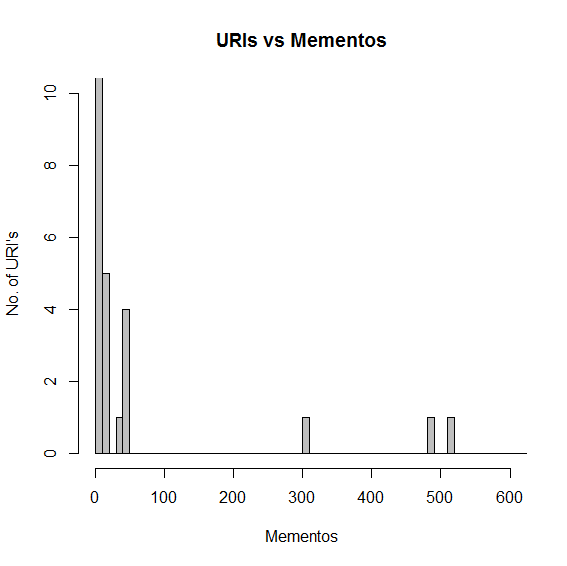
\includegraphics[scale=0.5]{plot1.png}
\caption{Histogram of URIs vs. number of Mementos for URIs with less than 600 Mementos }
\label{Hist 2}
\end{figure}
\begin{figure}
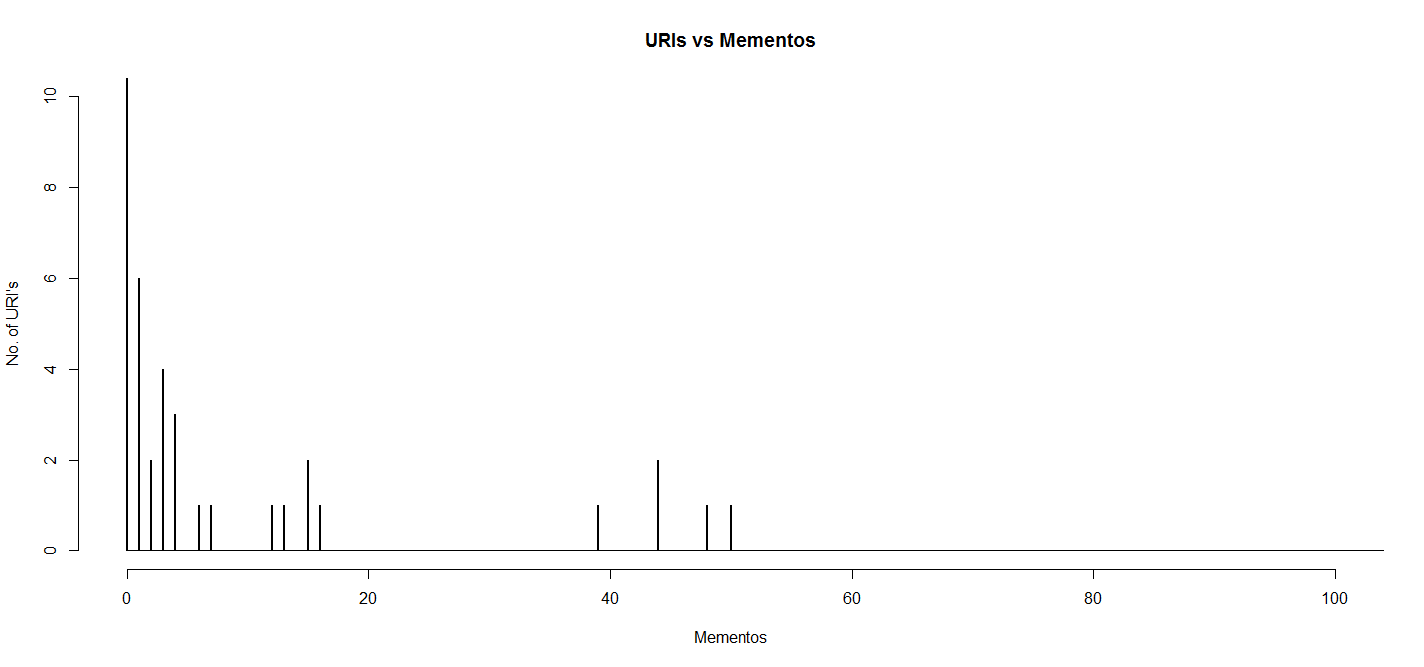
\includegraphics[scale=0.3]{plot3.png}
\caption{Histogram of URIs vs. number of Mementos for URIs with less than 100 Mementos and breaks inserted between each memento }
\label{Hist 3}
\end{figure}

\newpage
\section{Question 3}
\label{part3}
\begin{verbatim}
Estimate the age of each of the 1000 URIs using the "Carbon Date" tool:

http://ws-dl.blogspot.com/2013/04/2013-04-19-carbon-dating-web.html

Note: you'll have to download the tool and install; don't try to use the 
web service.  

For URIs that have > 0 Mementos and an estimated creation date,
create a graph with age (in days) on one axis and number of mementos
on the other.
\end{verbatim}

\newpage
\subsection{Answer}
``Carbon Date''  webservice gives the created date,modified date etc of a url .One url at a time.The tool however, can be used to run over a list of urls. 

Here we need all the urls which generate atleast one memento.We can get them using memcount.py of problem 2. Our first goal is to find the created date of the urls. File local.py outputs the created dates of all the 33 urls which were having atleast one memento.

We can use these dates and subtract them from the current date which gives the total number of days or Age of each uri.days.py does this job.

Now, we have number of days in one file(numberdays.txt) and number of mementos of each file in another url.We can plot a scatter plot with days on y axis and urls on x axis.The 
\lstinputlisting[language=Python,frame=single,caption={Python program for generating count of urls and mementos which have more than zero mementos}, label=lst:q3Query,captionpos=b,numbers=left,showspaces=false,showstringspaces=false,basicstyle=\footnotesize]{memcount.py}

\lstinputlisting[language=Python,frame=single,caption={Python program for extracting the created date of all the urls}, label=lst:q3Convert,captionpos=b,numbers=left,showspaces=false,showstringspaces=false,basicstyle=\footnotesize]{local.py}

\lstinputlisting[language=Python,frame=single,caption={Python program for calculating the ages by subtracting the created date from current date }, label=lst:q3Join,captionpos=b,numbers=left,showspaces=false,showstringspaces=false,basicstyle=\footnotesize]{days.py}

\subsubsection{ Results}
Graph shows an increasing curve .That is, those urls with less mementos have less age and those urls with more mementos have more age,which is the ideal situation.

\lstinputlisting[language=R,frame=single,caption={R program for generating the scatterplot for Question 3}, label=lst:q3R,captionpos=b,numbers=left,showspaces=false,showstringspaces=false,basicstyle=\footnotesize]{graphcmds.R}

\begin{figure}
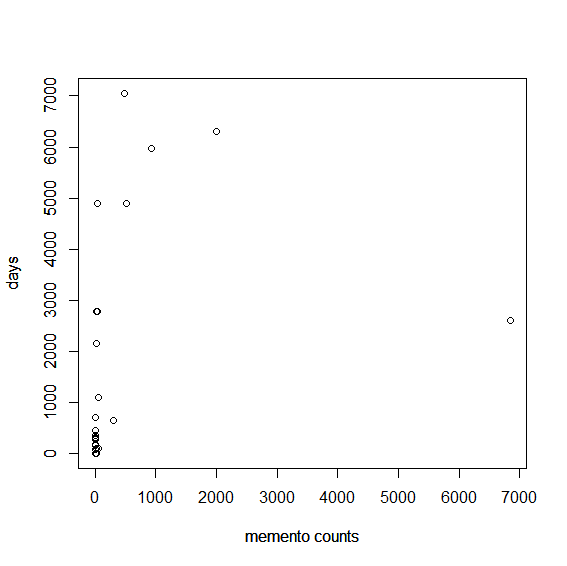
\includegraphics[scale=0.56]{graph1.png}
\caption{Number of Mementos vs. Days (Age of url) }

\end{figure}
\bibliographystyle{plain}
\bibliography{references}
\nocite {*} 

\end{document}


\newpage

